\documentclass[11pt,a4paper]{ivoa}
\input tthdefs

\title{Common Archive Observation Model}

\ivoagroup{Data Models}

\author[https://wiki.ivoa.net/twiki/bin/view/IVOA/PatrickDowler]{Patrick Dowler}

\editor{Patrick Dowler}
\editor{S\'everin Gaudet}

\previousversion[https://www.opencadc.org/caom2/]{CAOM-2.4}

\begin{document}
\begin{abstract}
???? Abstract ????
\end{abstract}


\section*{Acknowledgments}

???? Ack ????

\section*{Conformance-related definitions}

The words ``MUST'', ``SHALL'', ``SHOULD'', ``MAY'', ``RECOMMENDED'', and
``OPTIONAL'' (in upper or lower case) used in this document are to be
interpreted as described in IETF standard RFC2119 \citep{std:RFC2119}.

The \emph{Virtual Observatory (VO)} is a
general term for a collection of federated resources that can be used
to conduct astronomical research, education, and outreach.
The \href{https://www.ivoa.net}{International
Virtual Observatory Alliance (IVOA)} is a global
collaboration of separately funded projects to develop standards and
infrastructure that enable VO applications.


\section{Introduction}

The Common Archive Observation Model (CAOM) is a metadata model that describes
astronomical data stored in archives and make that data findable and accessible
(the first two concepts of the FAIR principles: Findable, Accessible, Interoperable,
Reusable). CAOM places no constraints on the format of the data itself and thus does 
not support or enable interoperable and reusable data.

\subsection{Role within the VO Architecture}

\begin{figure}
\centering

% As of ivoatex 1.2, the architecture diagram is generated by ivoatex in
% SVG; copy ivoatex/archdiag-full.xml to role_diagram.xml and throw out
% all lines not relevant to your standard.
% Notes don't generally need this.  If you don't copy role_diagram.xml,
% you must remove role_diagram.pdf from SOURCES in the Makefile.

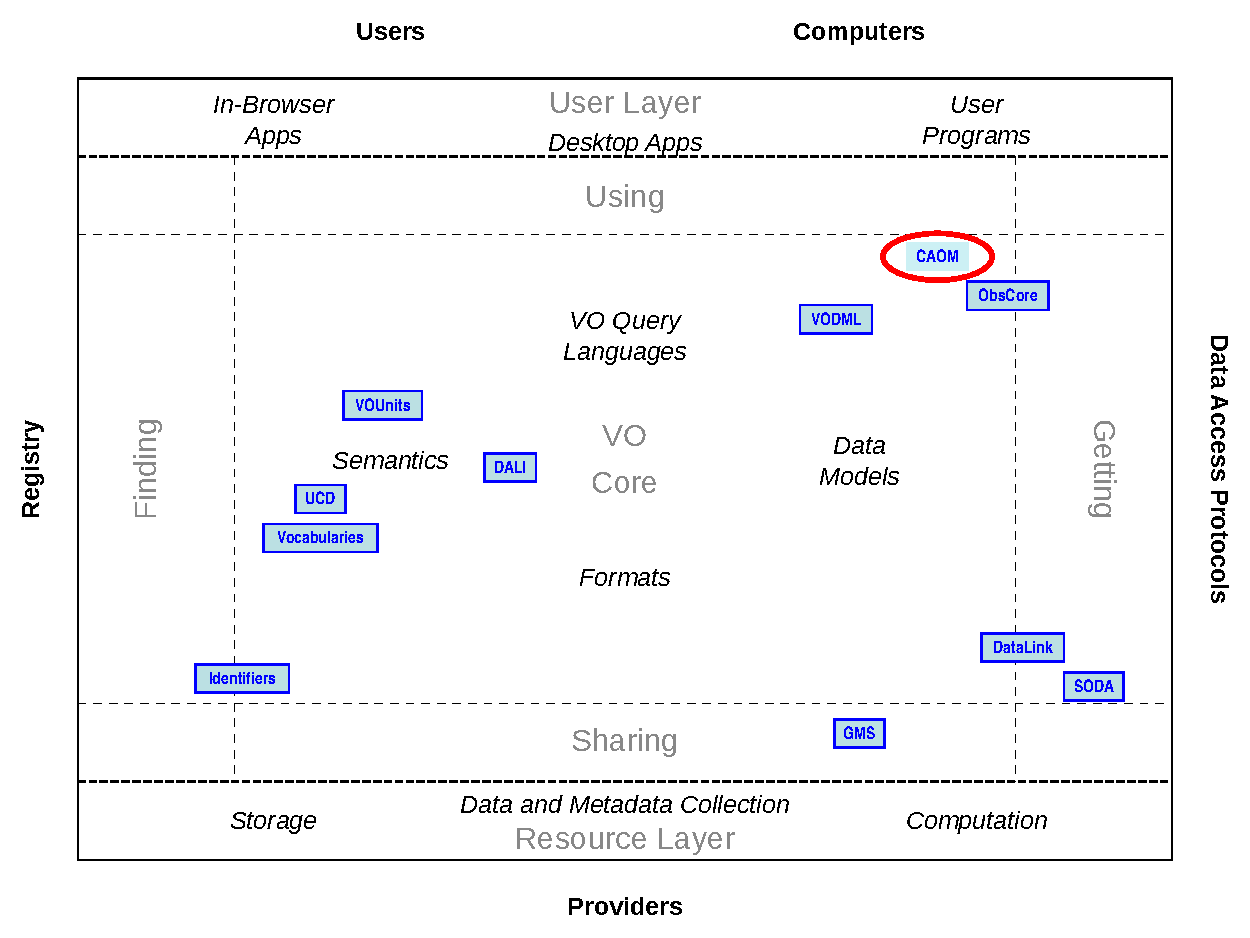
\includegraphics[width=0.9\textwidth]{role_diagram.pdf}
\caption{Architecture diagram for this document}
\label{fig:archdiag}
\end{figure}

Fig.~\ref{fig:archdiag} shows the role this document plays within the
IVOA architecture \citep{2021ivoa.spec.1101D}.

???? and so on, LaTeX as you know and love it. ????

\section{Use Cases}

TODO

\subsection{Describing Data}

The primary design goal of CAOM is to describe astronomical data so that 
users (astronomers) can query archives and discover data that is suitable
for a specific research goal or project. 

The metadata includes descriptive quantities to help users discover data, 
such as coverage in position, energy, and time, logical data types like 
images, spectra, and time series, and some some origin metadata like 
telescope, instrument, and proposal information.

The model also includes a structure that captures some of the important relationships 
between data products, such as different products of an observation that have had
different processing applied and new derived observations that are created by 
combining data from several other observations. CAOM also describes the way a
data product is made up of one or more physically stored components while remaining
loosely coupled with the storage system itself.

CAOM provides a transparent way to express data access rights so users can see
which data they have access to and even query for data that will soon be available.

Most importantly, new kinds of data products and areas of study sometimes require 
that the model must evolve (and new features) to better describe new data and enable
the queries that new research requires. CAOM has a well defined mechanism to support
evolution and still bring all legacy data forward with minimal effort.

\subsection{Implementation and Operations}

CAOM also supports a range of data management functions that make it implementable
and robust for large scale archive operations. The integrity of metadata that is 
created, stored, and accessed can be verified using a metadata checksum algorithm.
The metadata checksums can also be used to optimise interactions like database 
transactions and test database persistence and other forms of serialisation for
completeness and correctness.

The model is designed to support robust synchronisation of observation metadata 
between the origin and other mirror sites through modification timestamps and 
the use of metadata checksums to insure that metadata transport does not introduce
any corruption or incompleteless (details elsewhere ???).

\section{Model Overview}

\begin{figure}
\centering
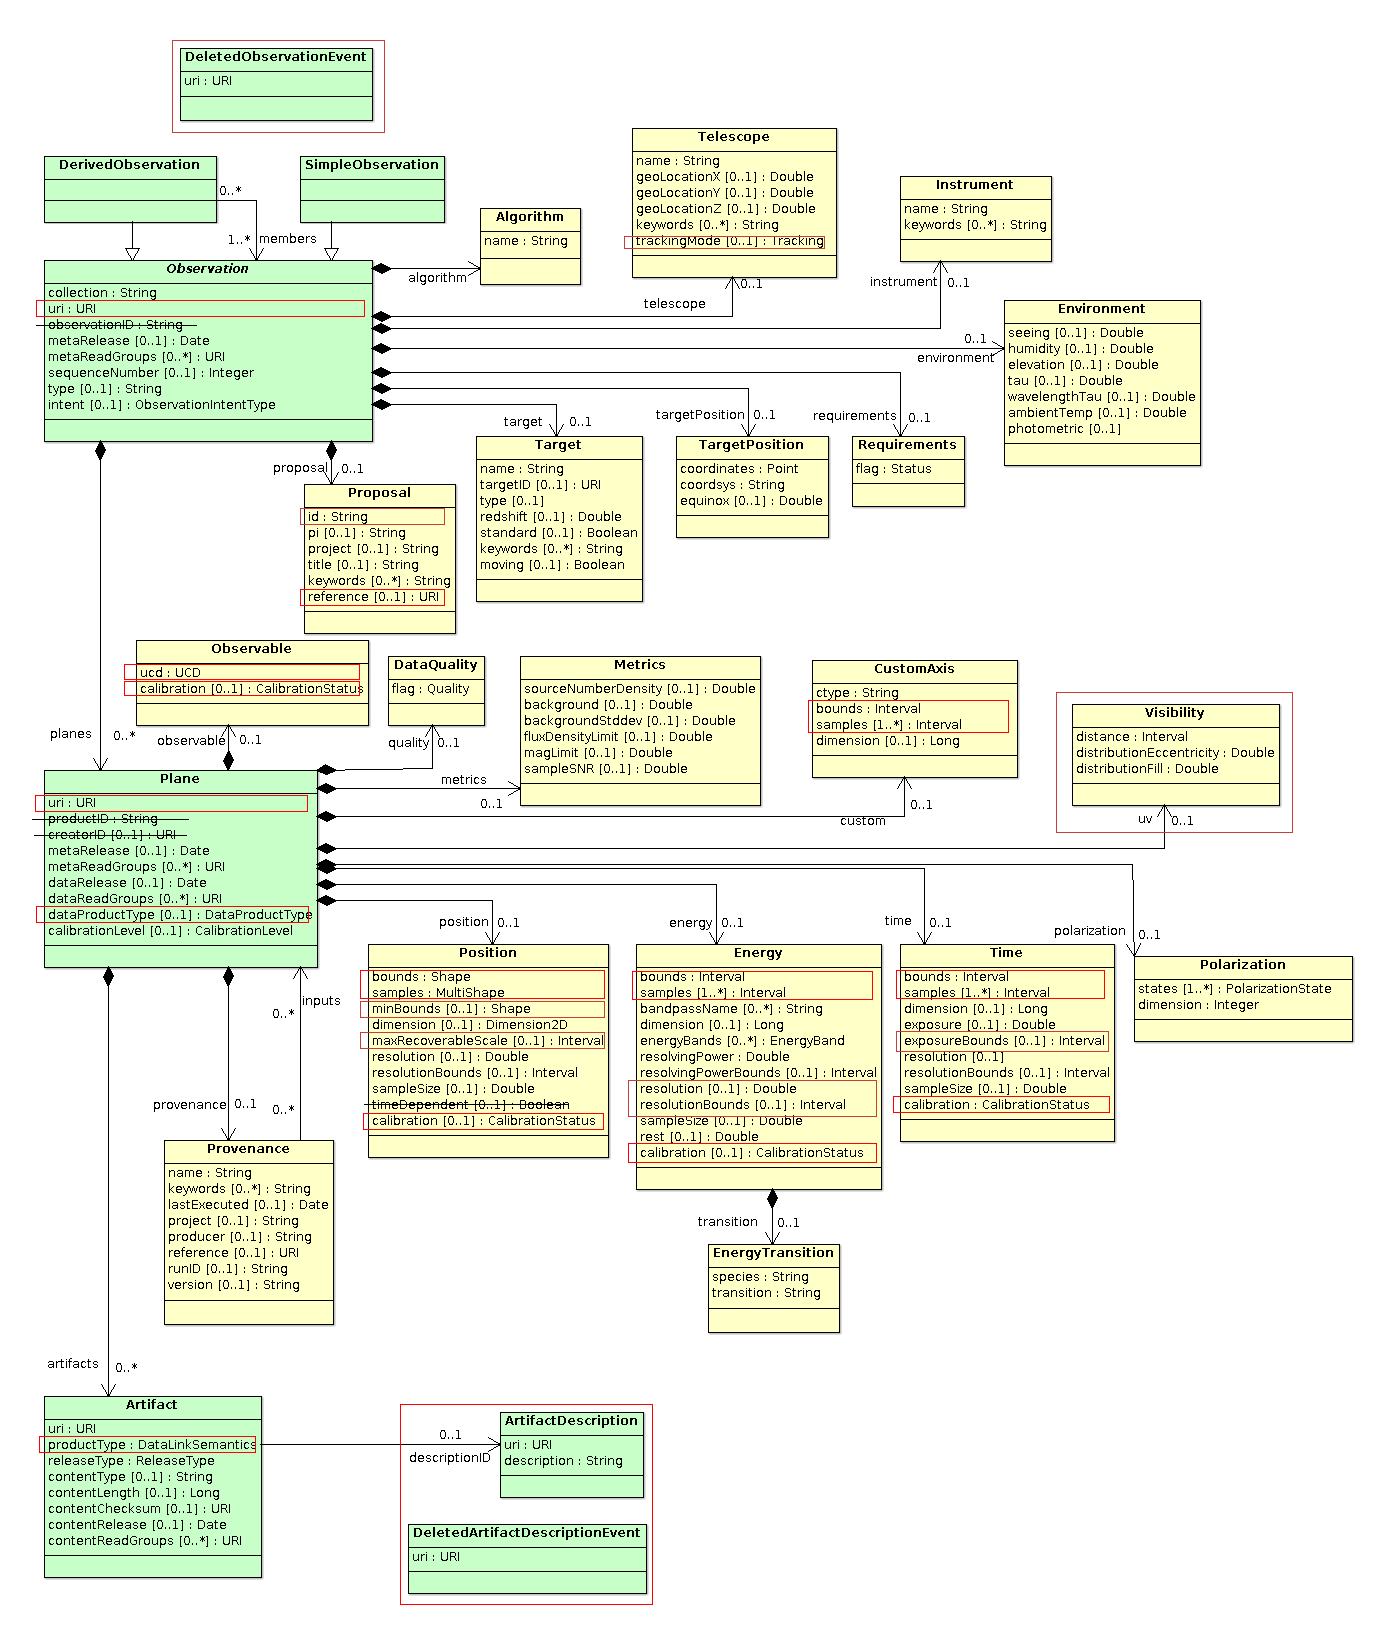
\includegraphics[width=0.9\textwidth]{src/uml/CAOM1core.png}
\caption{Main CAOM classes}
\label{fig:core}
\end{figure}

\subsection{Observation}

An Observation is the result of some activity to create data. Data acquisition by a 
telescope creates a SimpleObservation, usually with one Plane describing the raw 
data. Processing that creates a new observation (e.g. by combining mutliple independent
observations into a single product) creates a DerivedObservation with a set of member
observations. 

\subsection{Plane}

A Plane is a single data product within an Observation, usually with one or more
Artifact(s) that correspond to resources (usually files) that are stored. Processing
that transforms the data in a Plane in some fashion usually creates a new Plane in
the same observation. Common processing like calibration to remove the instrument
signature change the calibration level of the plane.

\subsection{Artifact}

An Artifact holds a reference to an externally stored resource: a file, a
database object (schema or table), a collection of files (directory), etc.

\subsection{ArtifactDescription}

An ArtifactDesciption is a human-readable description of an artifact. These
descriptions are intended to be shared across many artifacts curated by a single
operator; each artifact contains an optional reference to a description. The
primary intended use of these descriptions is to populate the description field
in a DataLink links response.

\subsection{Part}

A Part describes a logical subcomponent of an Artifact. For example, a single 
extension in a multi-extension FITS file, or a file inside a tar file would be parts
of such an Artifact. The meaning of Part depends on the type of resource that the
Artifact refers to, as described by the Artifact.contentType.

Note: Part is not shown in the UML diagrams. TBD: keep, deprecate, or remove?

\subsection{Chunk}

A Chunk describes a single data array using WCS (World Coordinate System) concepts. 

Note: Chunk is not shown in the UML diagrams. TBD: keep, deprecate or remove?

\subsection{DeletedObservationEvent}

Observation(s) are designed to support metadata sharing (synchronisation of instances
from a source site to a destination site). In some cases, observations are deleted at the 
source site; in that case, the source site would create a DeletedObservationEvent with the same 
entity identifier (Entity.id) and logical identifier (Observation.uri) so that other sites can
synchronise the event and perform the correct deletion locally.

\subsection{DeletedArtifactDescriptionEvent}

ArtifactDescription(s) are designed to support metadata sharing (synchronisation of instances
from a source site to a destination site). In some cases, descriptions are deleted at the 
source site; in that case, the source site would create a DeletedArtifactDescriptionEvent with 
the same entity identifier (Entity.id) and logical identifier (ArtifactDescription.uri) so that 
other sites can synchronise the event and perform the correct deletion locally.

\subsection{Data Types}
Some of the classes in the model are intended to be used as data types (e.g. columns
types in a database and exposed as such in a TAP service).

\begin{figure}
\centering
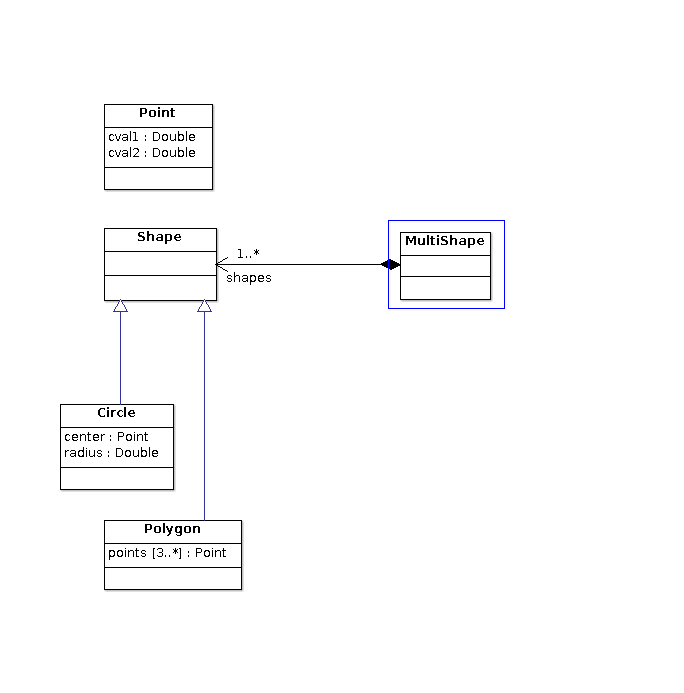
\includegraphics[width=0.9\textwidth]{src/uml/CAOM2datatypes.png}
\caption{CAOM Data Types}
\label{fig:datatypes}
\end{figure}

\subsection{Vocabularies}

CAOM uses a mixture of enumerations and vocabulary references. As it has evolved,
several concepts began as enumerations and were later converted to use a vocabulary
when it became clear that the IVOA Vocabularies process was a more appropriate way
to support the gradual evolution of set of concepts needed by the community.

\begin{figure}
\centering
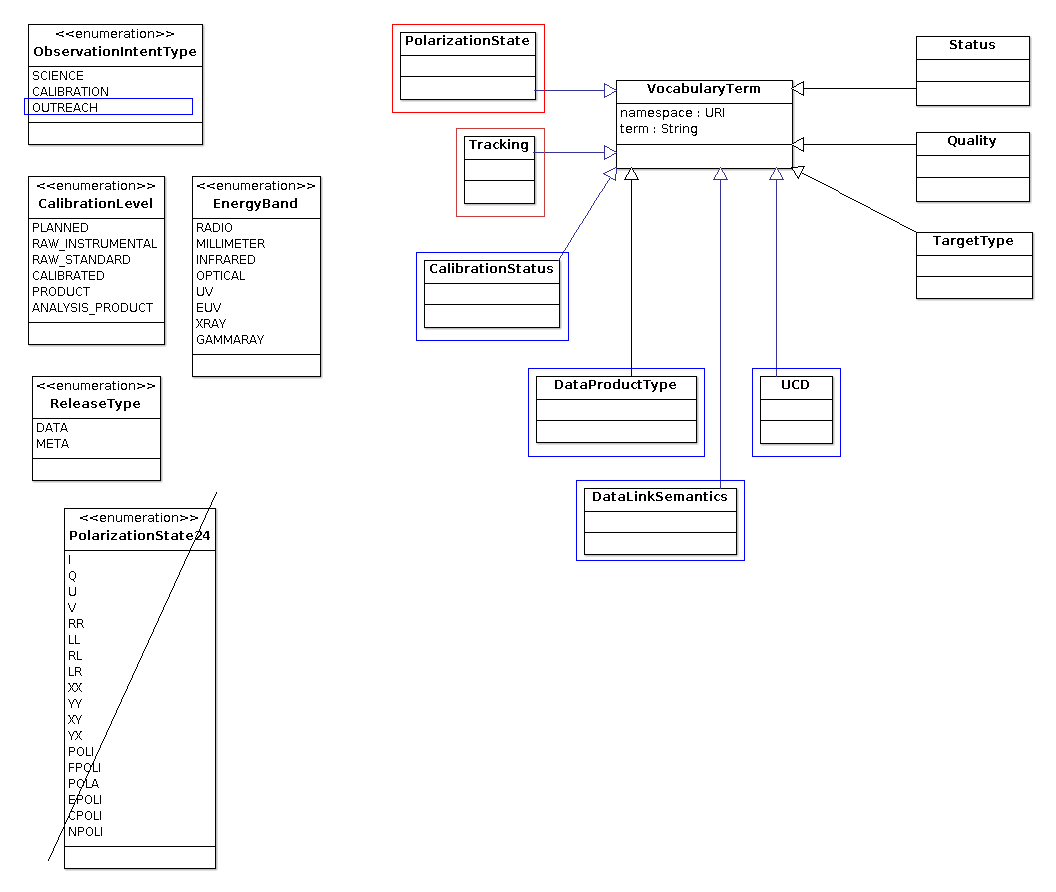
\includegraphics[width=0.9\textwidth]{src/uml/CAOM3vocabularies.png}
\caption{Enumerations and Vocabularies}
\label{fig:vocab}
\end{figure}

\subsection{Entity}

The Entity concept defines the common metadata necessary to persist and validate 
instances of classes within the model. Practically, the entity classes in the 
model are related by one-to-many composition and thus indicate a limit when
implementing (e.g. in a relational mapping, each entity has to be in a separate
table and one table per entity would be the minimum number of tables required 
to persist complete instances).

\begin{figure}
\centering
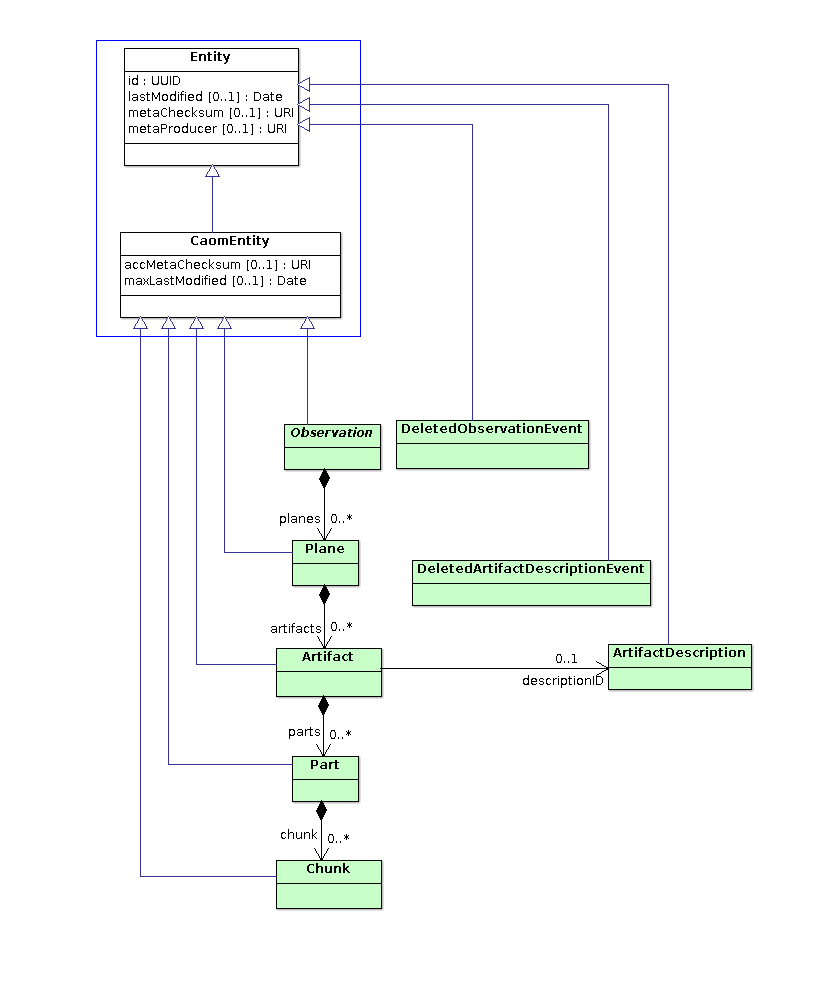
\includegraphics[width=0.9\textwidth]{src/uml/CAOM4entities.png}
\caption{CAOM Entities}
\label{fig:entity}
\end{figure}


% include external generated file so this tex doc is easy to edit

% -------------------------------------------
% Items to substitute into the ivoatex document template.
%
%\ivoagroup{Data Model Working Group}

%\title{Common Archive Observation Model}


%\author{Patrick Dowler}
    
%\author{Canadian Astronomy Data Centre}
    
% -------------------------------------------

\pagebreak
\section{Model: caom2 }
  
  % INSERT FIGURE HERE
  %\begin{figure}[h]
  %\begin{center}
  %  \includegraphics[width=\textwidth]{????.png}
  %  \caption{???}\label{fig:????}
  %\end{center}
  %\end{figure}

  a general purpose data model for use as the core data model of an astronomical data centre

  \subsection{Algorithm}
  \label{sect:Algorithm}
    The algorithm is the operation responsible for creating the observation. For a DerivedObservation, this is the algorithm that defines the intended set of members.

    \subsubsection{Algorithm.name}
      \textbf{vodml-id: Algorithm.name} \newline
      \textbf{type: \hyperref[sect:ivoa]{ivoa:string}} \newline
      \textbf{multiplicity: 1} \newline
      The algorithm name defines very high level categories of observations. See SimpleObservation and DerivedObservation for existing use. TBD: publish a list of acceptable values as a machine-readable vocabulary?

  \subsection{Artifact}
  \label{sect:Artifact}
    a physical product (typically a file)

    \subsubsection{Artifact.uri}
      \textbf{vodml-id: Artifact.uri} \newline
      \textbf{type: \hyperref[sect:ivoa]{ivoa:anyURI}} \newline
      \textbf{multiplicity: 1} \newline
      This identifier can be used to interact with an associated data management system. Existing usage: this is an internal identifier that an IVOA DataLink service can convert into a usable link to the data. TODO: There is an informal style used to make sure that these identifiers are globally unique and avoid collisions...

    \subsubsection{Artifact.uriBucket}
      \textbf{vodml-id: Artifact.uriBucket} \newline
      \textbf{type: \hyperref[sect:ivoa]{ivoa:string}} \newline
      \textbf{multiplicity: 1} \newline
      This is a short string of hexadecimal digits generated from the uri to support operational use cases (mainly: dividing workload to perform validation in parallel). The value is the first three characters of the hexadecimal representation of SHA-1 of the UTF-8 encoded bytes of the Observation.uri value. (NEW in CAOM-2.5)

    \subsubsection{Artifact.productType}
      \textbf{vodml-id: Artifact.productType} \newline
      \textbf{type: \hyperref[sect:DataLinkSemantics]{caom2:DataLinkSemantics}} \newline
      \textbf{multiplicity: 1} \newline
      This term describes the relationship of this Artifact to the parent Plane using IVOA DataLink semantics concepts.

    \subsubsection{Artifact.releaseType}
      \textbf{vodml-id: Artifact.releaseType} \newline
      \textbf{type: \hyperref[sect:ReleaseType]{caom2:ReleaseType}} \newline
      \textbf{multiplicity: 1} \newline
      This field indicates whether this artifact is treated as data or metadata when determining access permission. Existing usage: some collections have small previews (productType=thumbnail) that are considered metadata and are thus viewable by all users.

    \subsubsection{Artifact.contentType}
      \textbf{vodml-id: Artifact.contentType} \newline
      \textbf{type: \hyperref[sect:ivoa]{ivoa:string}} \newline
      \textbf{multiplicity: 0..1} \newline
      This field specifies the format of the resolved artifact: should be a MIME-type.

    \subsubsection{Artifact.contentLength}
      \textbf{vodml-id: Artifact.contentLength} \newline
      \textbf{type: dt:int64} \newline
      \textbf{multiplicity: 0..1} \newline
      This specifies the size of the stored artifact; for files, this is the file size.

    \subsubsection{Artifact.contentChecksum}
      \textbf{vodml-id: Artifact.contentChecksum} \newline
      \textbf{type: \hyperref[sect:ivoa]{ivoa:anyURI}} \newline
      \textbf{multiplicity: 0..1} \newline
      this is the checksum of the artifact data; the URI must conform to the pattern {algorithm}:{hex value}, for example: \begin{verbatim} md5:4be91751541fd804e7207663a0822f56 \end{verbatim}

    \subsubsection{Artifact.contentRelease}
      \textbf{vodml-id: Artifact.contentRelease} \newline
      \textbf{type: \hyperref[sect:ivoa]{ivoa:datetime}} \newline
      \textbf{multiplicity: 0..1} \newline
      This timestamp after which content for the artifact is public. If set, this value overrides the permission implied by the releaseType and Plane release dates. Existing usage: MAST?.

    \subsubsection{Artifact.contentReadGroups}
      \textbf{vodml-id: Artifact.contentReadGroups} \newline
      \textbf{type: \hyperref[sect:ivoa]{ivoa:anyURI}} \newline
      \textbf{multiplicity: 0..*} \newline
      Thsi is a set of groups that are allowed to access the content of this artifact. If set, thisd overrides the permission implied by the releaseType and PLane release groups. Existing usage: unknown.

    \subsubsection{Artifact.descriptionID}
      \textbf{vodml-id: Artifact.descriptionID} \newline
      \textbf{type: \hyperref[sect:ivoa]{ivoa:anyURI}} \newline
      \textbf{multiplicity: 0..1} \newline
      This is an identifier to refer to an ArtifactDescription entity (new in CAOM-2.5). Use case: provide standard descriptions for links in a DataLink response.

  \subsection{ArtifactDescription}
  \label{sect:ArtifactDescription}
    Ths entity provides a referenceable description of artifacts for use in DataLink responses (NEW in CAOM-2.5).

    \subsubsection{ArtifactDescription.uri}
      \textbf{vodml-id: ArtifactDescription.uri} \newline
      \textbf{type: \hyperref[sect:ivoa]{ivoa:anyURI}} \newline
      \textbf{multiplicity: 1} \newline
      This is the logical identifier for this description used to refer to it from an artifact. Anticipated usage: this is an internal identifier that an IVOA DataLink service can use to lookup a description. TODO: document the informal style also used for Artifact.uri to make sure that these identifiers are globally unique and avoid collisions.

    \subsubsection{ArtifactDescription.description}
      \textbf{vodml-id: Artifact.description} \newline
      \textbf{type: \hyperref[sect:ivoa]{ivoa:string}} \newline
      \textbf{multiplicity: 1} \newline
      The description is a human-readable description of an artifact.

  \subsection{CalibrationStatus}
  \label{sect:CalibrationStatus}
    This is a proposal for the creation of a IVOA calibration-status vocabulary. This vocabulary can be created using optional terms in the ObsCore standard to describe the calibration of each axis in the data separately. (NEW in CAOM-2.5)

  \subsection{CaomEntity (Abstract)}
  \label{sect:CaomEntity}
    This is an extension of the base Entity class to support accumulated metadata checksums and accumulated lastModified timestamps for entities with child entities.

    \subsubsection{CaomEntity.maxLastModified}
      \textbf{vodml-id: CaomEntity.maxLastModified} \newline
      \textbf{type: \hyperref[sect:ivoa]{ivoa:datetime}} \newline
      \textbf{multiplicity: 0..1} \newline
      The maximum last modification timestamp of this entity and all child entities is used to support incremental synchronization (of Observation instances). As with the instance lastModified timestamp above, this timestamp is intended to be set and/or updated when the entity is stored (e.g. in a database).

    \subsubsection{CaomEntity.accMetaChecksum}
      \textbf{vodml-id: CaomEntity.accMetaChecksum} \newline
      \textbf{type: \hyperref[sect:ivoa]{ivoa:anyURI}} \newline
      \textbf{multiplicity: 0..1} \newline
      accumulated checksum of the metadata of this entity and all child entities; The URI must conform to the pattern {algorithm}:{hex value}, for example: \begin{verbatim}md5:4be91751541fd804e7207663a0822f56.\end{verbatim} The accumulated checksum of an entity is computed by accumulating the byte representation of entity checksums in the following order: (1) the metaChecksum of the current entity, (2) the accMetaChecksum of all child entities accumulated in order of the child's Entity.id. For an entity with no children, the accMetaChecksum is derived only from the metaChecksum but it is not equal to it because it is a checksum of that checksum and not a checksum of the same metadata directly.

  \subsection{CustomAxis}
  \label{sect:CustomAxis}
    description of a custom coordinate axis (new in CAOM-2.4)

    \subsubsection{CustomAxis.ctype}
      \textbf{vodml-id: CustomAxis.ctype} \newline
      \textbf{type: \hyperref[sect:ivoa]{ivoa:string}} \newline
      \textbf{multiplicity: 1} \newline
      coordinate type code

    \subsubsection{CustomAxis.bounds}
      \textbf{vodml-id: CustomAxis.bounds} \newline
      \textbf{type: dt:Interval} \newline
      \textbf{multiplicity: 1} \newline
      custom coordinate coverage (cardinality changed in CAOM-2.5)

    \subsubsection{CustomAxis.samples}
      \textbf{vodml-id: CustomAxis.samples} \newline
      \textbf{type: dt:Interval} \newline
      \textbf{multiplicity: 1..*} \newline
      detailed custom coordinate coverage (refactored in CAOM-2.5)

    \subsubsection{CustomAxis.dimension}
      \textbf{vodml-id: CustomAxis.dimension} \newline
      \textbf{type: dt:int64} \newline
      \textbf{multiplicity: 0..1} \newline
      number of discrete samples (pixels) along custom axis

  \subsection{DataLinkSemantics}
  \label{sect:DataLinkSemantics}
    This is the IVOA DataLink Core vocabulary. (CHANGED in 2.5)

  \subsection{DataProductType}
  \label{sect:DataProductType}
    This is the IVOA product-type vocabulary that was extracted from the original ObsCore standard. (CHANGED in CAOM-2.5)

  \subsection{DataQuality}
  \label{sect:DataQuality}
    description of the data quality

    \subsubsection{DataQuality.flag}
      \textbf{vodml-id: DataQuality.flag} \newline
      \textbf{type: \hyperref[sect:Quality]{caom2:Quality}} \newline
      \textbf{multiplicity: 1} \newline
      flag indicating the data quality

  \subsection{DeletedArtifactDescriptionEvent}
  \label{sect:DeletedArtifactDescriptionEvent}
    an event signifiying that a previously persisted ArtifactDescription was deleted; this event can be synchronized to propagate deletions; the Entity.id of the event is equal to the Entity.id of the deleted observation and this identifier is used when performing deletions

    \subsubsection{DeletedArtifactDescriptionEvent.uri}
      \textbf{vodml-id: DeletedArtifactDescriptionEvent.uri} \newline
      \textbf{type: \hyperref[sect:ivoa]{ivoa:anyURI}} \newline
      \textbf{multiplicity: 1} \newline
      The logical identifier of the ArtifactDescription: the ArtifactDescription.uri value; this is for informational purposes only

  \subsection{DeletedObservationEvent}
  \label{sect:DeletedObservationEvent}
    an event signifiying that a previously persisted Observation was deleted; this event can be synchronized to propagate deletions; the Entity.id of the event is equal to the Entity.id of the deleted observation and this identifier is used when performing deletions

    \subsubsection{DeletedObservationEvent.uri}
      \textbf{vodml-id: DeletedObservationEvent.uri} \newline
      \textbf{type: \hyperref[sect:ivoa]{ivoa:anyURI}} \newline
      \textbf{multiplicity: 1} \newline
      The logical identifier of the Observation: the Observation.uri value; this is for informational purposes only

  \subsection{DerivedObservation}
  \label{sect:DerivedObservation}
    A derived observation is an observation created from one or more other observations. Examples of multiple members include: stacks of images combined to increase signal:noise ratio, mosaics combined to increase field-of-view, etc. Examples of single members: subset of comensurally observed data that is attributed/assigned to one proposal or project (with associated permissions).

    \subsubsection{DerivedObservation.members}
      \textbf{vodml-id: DerivedObservation.members} \newline
      \textbf{type: \hyperref[sect:ivoa]{ivoa:anyURI}} \newline
      \textbf{multiplicity: 0..*} \newline
      The members are the observations grouped together by the algorithm that defines the derivation. these are the intended components of the composite product, but actual inputs are described by the provenance. Members may be simple or derived observations (arbitrary heirarchy); derived observations with one or more members may be defined such that they only include a subset of each member (they are extracted from the progenitor). Observation.uri values are used here to refer to the member observations.

  \subsection{Dimension2D}
  \label{sect:Dimension2D}
    dimension (number of pixels) for a two-dimensional axis

    \subsubsection{Dimension2D.naxis1}
      \textbf{vodml-id: Dimension2D.naxis1} \newline
      \textbf{type: dt:int64} \newline
      \textbf{multiplicity: 1} \newline
      [TODO add description!]

    \subsubsection{Dimension2D.naxis2}
      \textbf{vodml-id: Dimension2D.naxis2} \newline
      \textbf{type: dt:int64} \newline
      \textbf{multiplicity: 1} \newline
      [TODO add description!]

  \subsection{Energy}
  \label{sect:Energy}
    description of the energy coverage and sampling of the data

    \subsubsection{Energy.bounds}
      \textbf{vodml-id: Energy.bounds} \newline
      \textbf{type: dt:Interval} \newline
      \textbf{multiplicity: 1} \newline
      simple outer bounds of energy coverage of the data (CHANGED cardinality in CAOM-2.5)

    \subsubsection{Energy.samples}
      \textbf{vodml-id: Energy.samples} \newline
      \textbf{type: dt:Interval} \newline
      \textbf{multiplicity: 1..*} \newline
      detailed energy coverage of the data (CHANGED in CAOM-2.5)

    \subsubsection{Energy.energyBands}
      \textbf{vodml-id: Energy.energyBands} \newline
      \textbf{type: \hyperref[sect:EnergyBand]{caom2:EnergyBand}} \newline
      \textbf{multiplicity: 0..*} \newline
      standard name of the energy regime(s) included in the data

    \subsubsection{Energy.dimension}
      \textbf{vodml-id: Energy.dimension} \newline
      \textbf{type: dt:int64} \newline
      \textbf{multiplicity: 0..1} \newline
      number of measurements (pixels) on the energy axis

    \subsubsection{Energy.resolvingPower}
      \textbf{vodml-id: Energy.resolvingPower} \newline
      \textbf{type: dt:double} \newline
      \textbf{multiplicity: 0..1} \newline
      mean spectral resolving power per pixel (relative resolution)

    \subsubsection{Energy.resolvingPowerBounds}
      \textbf{vodml-id: Energy.resolvingPowerBounds} \newline
      \textbf{type: dt:Interval} \newline
      \textbf{multiplicity: 0..1} \newline
      range of resolving power within the bounds (relative resolution)

    \subsubsection{Energy.resolution}
      \textbf{vodml-id: Energy.resolution} \newline
      \textbf{type: dt:double} \newline
      \textbf{multiplicity: 0..1} \newline
      mean absolute spectral resolution per pixel (new in CAOM-2.5)

    \subsubsection{Energy.resolutionBounds}
      \textbf{vodml-id: Energy.resolutionBounds} \newline
      \textbf{type: dt:Interval} \newline
      \textbf{multiplicity: 0..1} \newline
      range of absolute spectral resolution within the bounds (new in CAOM-2.5)

    \subsubsection{Energy.sampleSize}
      \textbf{vodml-id: Energy.sampleSize} \newline
      \textbf{type: dt:double} \newline
      \textbf{multiplicity: 0..1} \newline
      mean pixel size

    \subsubsection{Energy.bandpassName}
      \textbf{vodml-id: Energy.bandpassName} \newline
      \textbf{type: \hyperref[sect:ivoa]{ivoa:string}} \newline
      \textbf{multiplicity: 0..*} \newline
      telescope- and instrument-specific name for the energy band(s) included; multiple bands may be included if energies from all specified bands are included in the data (in the sense of union)

    \subsubsection{Energy.restwav}
      \textbf{vodml-id: Energy.rest} \newline
      \textbf{type: dt:double} \newline
      \textbf{multiplicity: 0..1} \newline
      rest energy of the target energy transition (name changed in CAOM-2.5)

    \subsubsection{Energy.calibration}
      \textbf{vodml-id: Energy.calibration} \newline
      \textbf{type: \hyperref[sect:CalibrationStatus]{caom2:CalibrationStatus}} \newline
      \textbf{multiplicity: 0..1} \newline
      term describing the calibration of the energy axis values (new in CAOM-2.5)

    \subsubsection{Energy.transition}
      \textbf{vodml-id: Energy.transition} \newline
      \textbf{type: \hyperref[sect:EnergyTransition]{caom2:EnergyTransition}} \newline
      \textbf{multiplicity: 0..1} \newline
      target energy transition for this data

  \subsection{EnergyTransition}
  \label{sect:EnergyTransition}
    [TODO add description!]

    \subsubsection{EnergyTransition.species}
      \textbf{vodml-id: EnergyTransition.species} \newline
      \textbf{type: \hyperref[sect:ivoa]{ivoa:string}} \newline
      \textbf{multiplicity: 1} \newline
      TODO

    \subsubsection{EnergyTransition.transition}
      \textbf{vodml-id: EnergyTransition.transition} \newline
      \textbf{type: \hyperref[sect:ivoa]{ivoa:string}} \newline
      \textbf{multiplicity: 1} \newline
      TODO

  \subsection{Entity (Abstract)}
  \label{sect:Entity}
    This is a base class to persistence. The entity attributes are generally set or updated by persistence implementations.

    \subsubsection{Entity.id}
      \textbf{vodml-id: Entity.id} \newline
      \textbf{type: dt:uuid} \newline
      \textbf{multiplicity: 1} \newline
      The id is a globally unique identifier (primary key) for an instance.

    \subsubsection{Entity.lastModified}
      \textbf{vodml-id: Entity.lastModified} \newline
      \textbf{type: \hyperref[sect:ivoa]{ivoa:datetime}} \newline
      \textbf{multiplicity: 0..1} \newline
      The timestamp of last modification of this entity tracks changes in metadata and supports incremental operations. The timestamp is intended to be set and/or updated when the entity is stored (e.g. in a database).

    \subsubsection{Entity.metaChecksum}
      \textbf{vodml-id: Entity.metaChecksum} \newline
      \textbf{type: \hyperref[sect:ivoa]{ivoa:anyURI}} \newline
      \textbf{multiplicity: 0..1} \newline
      This checksum of the metadata in this entity signals a change in the metadata of an instance and supports validation (e.g. to compare metadata before and after serialisation or persistence). A change in the metaChecksum can also be used to optimise operations like updating a row in the database only when the metaChecksum changed. A change in metaChecksum normally triggers a change in the lastModified timestamp. The URI must conform to the pattern {algorithm}:{hex value}, for example: \begin{verbatim}md5:4be91751541fd804e7207663a0822f56.\end{verbatim} The checksum of an entity is computed by accumulating byte representation of individual metadata values in the following order: (1) Entity.id for entities, (2) Entity.metaProducer, (3) state fields in alphabetic order (foo.a comes before foo.b) and using depth-first recursion (foo.abc.x comes before foo.def). The lastModified timestamp is not included in the metaChecksum calculation. Null values are ignored so that the addition of new fields in future versions will not change/invalidate existing checksums. Non-null values are converted to bytes as follows: \begin{itemize} \item string: UTF-8 encoded bytes \item URI: UTF-8 encoded bytes of the string representation \item VocabularyTerm: UTF-8 encoded bytes of the term (do not include the namespace) \item enumeration: the literal value converted to bytes \item float: IEEE754 single (4 bytes) \item double: IEEE754 double (8 bytes) \item boolean: convert to single byte, false=0, true=1 (1 byte) \item byte: as-is (1 byte) \item short: (2 bytes, network byte order == big endian)) \item integer: (4 bytes, network byte order == big endian) \item long: (8 bytes, network byte order == big endian) \item date: treat as a long (milliseconds since 1970-01-01 00:00:00 UTC) \end{itemize} TODO: truncatedDates=false, digestFieldNames=true, digestFieldnamesLowerCase=true TODO: external data model components: recursion or specify conversion above (interval, point, shape, multishape)

    \subsubsection{Entity.metaProducer}
      \textbf{vodml-id: Entity.metaProducer} \newline
      \textbf{type: \hyperref[sect:ivoa]{ivoa:anyURI}} \newline
      \textbf{multiplicity: 0..1} \newline
      This identifier is used to identify the tools used to produce the metadata. It also implicitly applies to child entities with null metaProducer. The form of the URI is not specified; implementations are free to use this to track metadata curation. For example, a pattern like {organisation}:{software name}-{version} is useful to support a variety of operational uses: query for metadata created by a version with a known bug or query for metadata created by an older version of the software and perform updates.

  \subsection{Environment}
  \label{sect:Environment}
    The environment is a collection of measured quantities that characterise the conditions when the observation was created.

    \subsubsection{Environment.name}
      \textbf{vodml-id: Environment.seeing} \newline
      \textbf{type: dt:double} \newline
      \textbf{multiplicity: 0..1} \newline
      The seeing is a measure of the atmospheric distortion: full-width-half-max of a point source.

    \subsubsection{Environment.humidity}
      \textbf{vodml-id: Environment.humidity} \newline
      \textbf{type: dt:double} \newline
      \textbf{multiplicity: 0..1} \newline
      The humidity is a meaure of the fractional relative humidity [0,1].

    \subsubsection{Environment.elevation}
      \textbf{vodml-id: Environment.elevation} \newline
      \textbf{type: dt:double} \newline
      \textbf{multiplicity: 0..1} \newline
      The elevation is the angular elevation above the horizon [0,90].

    \subsubsection{Environment.tau}
      \textbf{vodml-id: Environment.tau} \newline
      \textbf{type: dt:double} \newline
      \textbf{multiplicity: 0..1} \newline
      Tau is a measure of the opacity of the atmosphere [0,1].

    \subsubsection{Environment.wavelengthTau}
      \textbf{vodml-id: Environment.wavelengthTau} \newline
      \textbf{type: dt:double} \newline
      \textbf{multiplicity: 0..1} \newline
      The tau (opacity) was measured at this wavelength.

    \subsubsection{Environment.ambientTemp}
      \textbf{vodml-id: Environment.ambientTemp} \newline
      \textbf{type: dt:double} \newline
      \textbf{multiplicity: 0..1} \newline
      The ambient temperature is a measurement of the typical temperature at/in the telescope.

    \subsubsection{Environment.photometric}
      \textbf{vodml-id: Environment.photometric} \newline
      \textbf{type: \hyperref[sect:ivoa]{ivoa:boolean}} \newline
      \textbf{multiplicity: 0..1} \newline
      The photometric flag is an indicator that flux and/or color calibration is stable.

  \subsection{Instrument}
  \label{sect:Instrument}
    The instrument is the device that captures, aggregates, and digitise the signal from the telescope while creating an observation. An instrument could be physical hardware at a telescope (for empirical data) or software that generates it (for simulated data).

    \subsubsection{Instrument.name}
      \textbf{vodml-id: Instrument.name} \newline
      \textbf{type: \hyperref[sect:ivoa]{ivoa:string}} \newline
      \textbf{multiplicity: 1} \newline
      common name for the instrument

    \subsubsection{Instrument.keywords}
      \textbf{vodml-id: Instrument.keywords} \newline
      \textbf{type: \hyperref[sect:ivoa]{ivoa:string}} \newline
      \textbf{multiplicity: 0..*} \newline
      Additional keywords describe the instrument or instrument configuration at the time of observation. Keywords cannot contain the pipe (|) character: it is reserved for use in persistence systems (e.g. to store all keywords in a single column in a table).

  \subsection{Metrics}
  \label{sect:Metrics}
    collection of measured quantities that describe the content of the data

    \subsubsection{Metrics.sourceNumberDensity}
      \textbf{vodml-id: Metrics.sourceNumberDensity} \newline
      \textbf{type: dt:double} \newline
      \textbf{multiplicity: 0..1} \newline
      number of sources detected per unit area

    \subsubsection{Metrics.background}
      \textbf{vodml-id: Metrics.background} \newline
      \textbf{type: dt:double} \newline
      \textbf{multiplicity: 0..1} \newline
      background level

    \subsubsection{Metrics.backgroundStddev}
      \textbf{vodml-id: Metrics.backgroundStddev} \newline
      \textbf{type: dt:double} \newline
      \textbf{multiplicity: 0..1} \newline
      standard deviation in the background level

    \subsubsection{Metrics.fluxDensityLimit}
      \textbf{vodml-id: Metrics.fluxDensityLimit} \newline
      \textbf{type: dt:double} \newline
      \textbf{multiplicity: 0..1} \newline
      flux density with a signal:noise ratio of 10

    \subsubsection{Metrics.magLimit}
      \textbf{vodml-id: Metrics.magLimit} \newline
      \textbf{type: dt:double} \newline
      \textbf{multiplicity: 0..1} \newline
      magnitude with a signal:noise ratio of 10

    \subsubsection{Metrics.sampleSNR}
      \textbf{vodml-id: Metrics.sampleSNR} \newline
      \textbf{type: dt:double} \newline
      \textbf{multiplicity: 0..1} \newline
      signal:noise ratio for a representative subset of samples

  \subsection{Observable}
  \label{sect:Observable}
    description of the sample (pixel) values

    \subsubsection{Observable.ucd}
      \textbf{vodml-id: Observable.ucd} \newline
      \textbf{type: \hyperref[sect:UCD]{caom2:UCD}} \newline
      \textbf{multiplicity: 1} \newline
      Unified Content Descriptor (UCD) that says what kind of quantity is stored

    \subsubsection{Observable.calibration}
      \textbf{vodml-id: Observable.calibration} \newline
      \textbf{type: \hyperref[sect:CalibrationStatus]{caom2:CalibrationStatus}} \newline
      \textbf{multiplicity: 0..1} \newline
      term describing the calibration of the observable values

  \subsection{Observation (Abstract)}
  \label{sect:Observation}
    The observation is the top-level metadata structure that describes astronomical data in a data collection.

    \subsubsection{Observation.collection}
      \textbf{vodml-id: Observation.collection} \newline
      \textbf{type: \hyperref[sect:ivoa]{ivoa:string}} \newline
      \textbf{multiplicity: 1} \newline
      The name of the data collection to which this observation belongs.

    \subsubsection{Observation.uri}
      \textbf{vodml-id: Observation.uri} \newline
      \textbf{type: \hyperref[sect:ivoa]{ivoa:anyURI}} \newline
      \textbf{multiplicity: 1} \newline
      A unique logical identifier for this observation. (NEW in CAOM-2.5) TODO: limit this to one of two forms that support use cases?

    \subsubsection{Observation.uriBucket}
      \textbf{vodml-id: Observation.uriBucket} \newline
      \textbf{type: \hyperref[sect:ivoa]{ivoa:string}} \newline
      \textbf{multiplicity: 1} \newline
      This is a short string of hexadecimal digits generated from the uri to support operational use cases (mainly: dividing workload to perform validation in parallel). The value is the first three characters of the hexadecimal representation of SHA-1 of the UTF-8 encoded bytes of the Observation.uri value. (NEW in CAOM-2.5)

    \subsubsection{Observation.metaRelease}
      \textbf{vodml-id: Observation.metaRelease} \newline
      \textbf{type: \hyperref[sect:ivoa]{ivoa:datetime}} \newline
      \textbf{multiplicity: 0..1} \newline
      This timestamp specifies the point where the metadata for the observation instance is public (can be viewed by anonymous users). A null value means the metadata is nont public.

    \subsubsection{Observation.sequenceNumber}
      \textbf{vodml-id: Observation.sequenceNumber} \newline
      \textbf{type: dt:int32} \newline
      \textbf{multiplicity: 0..1} \newline
      a collection-specific sequence number for observations; re-use or reset is collection specific

    \subsubsection{Observation.type}
      \textbf{vodml-id: Observation.type} \newline
      \textbf{type: \hyperref[sect:ivoa]{ivoa:string}} \newline
      \textbf{multiplicity: 0..1} \newline
      This describes the general purpose of observation (e.g. FITS OBSTYPE keyword). Existing usage is usually OBJECT for intent = science and other values for intent = calibration.

    \subsubsection{Observation.intent}
      \textbf{vodml-id: Observation.intent} \newline
      \textbf{type: \hyperref[sect:ObservationIntentType]{caom2:ObservationIntentType}} \newline
      \textbf{multiplicity: 1} \newline
      This is an enumeration that describes the intent of the original creator of the observation.

    \subsubsection{Observation.metaReadGroups}
      \textbf{vodml-id: Observation.metaReadGroups} \newline
      \textbf{type: \hyperref[sect:ivoa]{ivoa:anyURI}} \newline
      \textbf{multiplicity: 0..*} \newline
      This is a set of groups with read permission on observation metadata for cases when the metadata is non-public (see metaRelease above).

    \subsubsection{Observation.algorithm}
      \textbf{vodml-id: Observation.algorithm} \newline
      \textbf{type: \hyperref[sect:Algorithm]{caom2:Algorithm}} \newline
      \textbf{multiplicity: 1} \newline
      This provides information about the algorithm or process that created this observation.

    \subsubsection{Observation.telescope}
      \textbf{vodml-id: Observation.telescope} \newline
      \textbf{type: \hyperref[sect:Telescope]{caom2:Telescope}} \newline
      \textbf{multiplicity: 0..1} \newline
      Information about the telescope or facility where this observation was created.

    \subsubsection{Observation.instrument}
      \textbf{vodml-id: Observation.instrument} \newline
      \textbf{type: \hyperref[sect:Instrument]{caom2:Instrument}} \newline
      \textbf{multiplicity: 0..1} \newline
      Information about the instrument or detector used to acquire the data.

    \subsubsection{Observation.environment}
      \textbf{vodml-id: Observation.environment} \newline
      \textbf{type: \hyperref[sect:Environment]{caom2:Environment}} \newline
      \textbf{multiplicity: 0..1} \newline
      Information about the environmental conditions at the time of observation.

    \subsubsection{Observation.proposal}
      \textbf{vodml-id: Observation.Proposal} \newline
      \textbf{type: \hyperref[sect:Proposal]{caom2:Proposal}} \newline
      \textbf{multiplicity: 0..1} \newline
      Information about the science proposal that motivated the creation of this observation.

    \subsubsection{Observation.target}
      \textbf{vodml-id: Observation.target} \newline
      \textbf{type: \hyperref[sect:Target]{caom2:Target}} \newline
      \textbf{multiplicity: 0..1} \newline
      Information about the intended target of the observation.

    \subsubsection{Observation.targetPosition}
      \textbf{vodml-id: Observation.targetPosition} \newline
      \textbf{type: \hyperref[sect:TargetPosition]{caom2:TargetPosition}} \newline
      \textbf{multiplicity: 0..1} \newline
      Information about the intended target position for this observation. This may differ from the coordinates of the target object itself.

    \subsubsection{Observation.requirements}
      \textbf{vodml-id: Observation.requirements} \newline
      \textbf{type: \hyperref[sect:Requirements]{caom2:Requirements}} \newline
      \textbf{multiplicity: 0..1} \newline
      Information about the observational requirements specified by the observer or proposal and whether this observation satisfies those requirements.

    \subsubsection{Observation.planes}
      \textbf{vodml-id: Observation.planes} \newline
      \textbf{type: \hyperref[sect:Plane]{caom2:Plane}} \newline
      \textbf{multiplicity: 0..*} \newline
      The planes within an observation are the different data products that are produced from the observation. For SimpleObservation, there are usually different planes for raw data, calibrated data, etc.

  \subsection{Plane}
  \label{sect:Plane}
    A plane is a component of an observation that describes one product of the observation.

    \subsubsection{Plane.uri}
      \textbf{vodml-id: Plane.uri} \newline
      \textbf{type: \hyperref[sect:ivoa]{ivoa:anyURI}} \newline
      \textbf{multiplicity: 0..1} \newline
      A unique logical identifier for this plane. Values of this identifier are used in Plane.provenance.inputs to form a reference from a product to it's progenitors. TODO: limit this to one of two forms that support use cases? (NEW in CAOM-2.5)

    \subsubsection{Plane.metaRelease}
      \textbf{vodml-id: Plane.metaRelease} \newline
      \textbf{type: \hyperref[sect:ivoa]{ivoa:datetime}} \newline
      \textbf{multiplicity: 0..1} \newline
      This timestamp specifies the point where the metadata for the plane instance is public (can be viewed by anonymous users). A null value means the metadata is not public. The metaRelease timestamp applies to the plane metadata itself and to all artifacts with releaseType=meta.

    \subsubsection{Plane.metaReadGroups}
      \textbf{vodml-id: Plane.metaReadGroups} \newline
      \textbf{type: \hyperref[sect:ivoa]{ivoa:anyURI}} \newline
      \textbf{multiplicity: 0..*} \newline
      This is a set of groups with read permission on plane metadata for cases when the metadata is non-public (see metaRelease above).

    \subsubsection{Plane.dataRelease}
      \textbf{vodml-id: Plane.dataRelease} \newline
      \textbf{type: \hyperref[sect:ivoa]{ivoa:datetime}} \newline
      \textbf{multiplicity: 0..1} \newline
      This timestamp specifies the point where the metadata for the plane instance is public (can be viewed by anonymous users). A null value means the metadata is not public. The dataRelease timestamp applies to all artifacts with releaseType=data.

    \subsubsection{Plane.dataReadGroups}
      \textbf{vodml-id: Plane.dataReadGroups} \newline
      \textbf{type: \hyperref[sect:ivoa]{ivoa:anyURI}} \newline
      \textbf{multiplicity: 0..*} \newline
      This is a set of groups with read permission on plane data for cases when the data is non-public (see dataRelease above).

    \subsubsection{Plane.calibrationLevel}
      \textbf{vodml-id: Plane.calibrationLevel} \newline
      \textbf{type: \hyperref[sect:CalibrationLevel]{caom2:CalibrationLevel}} \newline
      \textbf{multiplicity: 0..1} \newline
      This describes the degree to which the data is calibrated; it is equivalent to the ObsCore calibration level field.

    \subsubsection{Plane.dataProductType}
      \textbf{vodml-id: Plane.dataProductType} \newline
      \textbf{type: \hyperref[sect:DataProductType]{caom2:DataProductType}} \newline
      \textbf{multiplicity: 0..1} \newline
      This describes the logical type of data for this product; it is equivalent to the ObsCore data product type field.

    \subsubsection{Plane.observable}
      \textbf{vodml-id: Plane.observable} \newline
      \textbf{type: \hyperref[sect:Observable]{caom2:Observable}} \newline
      \textbf{multiplicity: 0..1} \newline
      The observable describes the quantity stored in the sample (pixel) values

    \subsubsection{Plane.quality}
      \textbf{vodml-id: Plane.quality} \newline
      \textbf{type: \hyperref[sect:DataQuality]{caom2:DataQuality}} \newline
      \textbf{multiplicity: 0..1} \newline
      This is a flag that indicates the quality of the data. Existing usage is that this is only assigned when there is something wrong with the data and the quality flag indicates roughly what is wrong.

    \subsubsection{Plane.metrics}
      \textbf{vodml-id: Plane.metrics} \newline
      \textbf{type: \hyperref[sect:Metrics]{caom2:Metrics}} \newline
      \textbf{multiplicity: 0..1} \newline
      Metrics are measured quantities that describe the content rather than the characteristics of the product.

    \subsubsection{Plane.position}
      \textbf{vodml-id: Plane.position} \newline
      \textbf{type: \hyperref[sect:Position]{caom2:Position}} \newline
      \textbf{multiplicity: 0..1} \newline
      Information about the positional coverage and sampling of the data.

    \subsubsection{Plane.energy}
      \textbf{vodml-id: Plane.energy} \newline
      \textbf{type: \hyperref[sect:Energy]{caom2:Energy}} \newline
      \textbf{multiplicity: 0..1} \newline
      Information about the energy coverage and sampling of the data.

    \subsubsection{Plane.time}
      \textbf{vodml-id: Plane.time} \newline
      \textbf{type: \hyperref[sect:Time]{caom2:Time}} \newline
      \textbf{multiplicity: 0..1} \newline
      Information about the time coverage and sampling of the data.

    \subsubsection{Plane.polarization}
      \textbf{vodml-id: Plane.polarization} \newline
      \textbf{type: \hyperref[sect:Polarization]{caom2:Polarization}} \newline
      \textbf{multiplicity: 0..1} \newline
      Information about the polarization state(s) of the data.

    \subsubsection{Plane.custom}
      \textbf{vodml-id: Plane.custom} \newline
      \textbf{type: \hyperref[sect:CustomAxis]{caom2:CustomAxis}} \newline
      \textbf{multiplicity: 0..1} \newline
      Information about the a single custom axis and sampling of the data. Since different custom coordinate types can be used with different planes, instances of CustomAxis can only be compared sensibly if they have the same coordinate type. Existing usage is experimental: Faraday Depth or Rotation Measure axes in radio data cubes.

    \subsubsection{Plane.uv}
      \textbf{vodml-id: Plane.uv} \newline
      \textbf{type: \hyperref[sect:Visibility]{caom2:Visibility}} \newline
      \textbf{multiplicity: 0..1} \newline
      Information about the UV plane coverage and sampling of the data for interferometric observations.

    \subsubsection{Plane.provenance}
      \textbf{vodml-id: Plane.provenance} \newline
      \textbf{type: \hyperref[sect:Provenance]{caom2:Provenance}} \newline
      \textbf{multiplicity: 0..1} \newline
      The provenance provides a description how the plane was created and the direct input planes that were used. This is a single-step provenance and not a complete description of all activities that led to this product.

    \subsubsection{Plane.artifacts}
      \textbf{vodml-id: Plane.artifacts} \newline
      \textbf{type: \hyperref[sect:Artifact]{caom2:Artifact}} \newline
      \textbf{multiplicity: 0..*} \newline
      This is the set of component artifacts belonging to this plane.

  \subsection{Polarization}
  \label{sect:Polarization}
    description of polarization measurements included in the data

    \subsubsection{Polarization.states}
      \textbf{vodml-id: Polarization.states} \newline
      \textbf{type: \hyperref[sect:PolarizationState]{caom2:PolarizationState}} \newline
      \textbf{multiplicity: 1..*} \newline
      standard polarization states included (CHANGED cardinality in CAOM-2.5)

    \subsubsection{Polarization.dimension}
      \textbf{vodml-id: Polarization.dimension} \newline
      \textbf{type: dt:int32} \newline
      \textbf{multiplicity: 0..1} \newline
      number of polarization states included

  \subsection{PolarizationState}
  \label{sect:PolarizationState}
    This is a proposed vocabulary to specify constants for the PolarizationState. Existing usage includes terms from the ObsCore polarization states list, plus some extra terms derived from community usage and proposals. (CHANGED from enumeration in CAOM-2.5)

  \subsection{Position}
  \label{sect:Position}
    description of the position coverage and sampling of the data

    \subsubsection{Position.bounds}
      \textbf{vodml-id: Position.bounds} \newline
      \textbf{type: dt:Shape} \newline
      \textbf{multiplicity: 1} \newline
      spatial boundary that includes the data (CHANGED cardinality in CAOM-2.5)

    \subsubsection{Position.samples}
      \textbf{vodml-id: Position.samples} \newline
      \textbf{type: dt:MultiShape} \newline
      \textbf{multiplicity: 1} \newline
      detailed sub-samples of the bounds (CHANGED in CAOM-2.5)

    \subsubsection{Position.minBounds}
      \textbf{vodml-id: Position.minBounds} \newline
      \textbf{type: dt:Shape} \newline
      \textbf{multiplicity: 0..1} \newline
      minimum spatial boundary that includes the data; this value is smaller than the bounds (maximum) when the field-of-view varies because it is dependent on another axis (usually energy) (new in CAOM-2.5)

    \subsubsection{Position.dimension}
      \textbf{vodml-id: Position.dimension} \newline
      \textbf{type: \hyperref[sect:Dimension2D]{caom2:Dimension2D}} \newline
      \textbf{multiplicity: 0..1} \newline
      number of separate measurements (pixels) along each axis

    \subsubsection{Position.maxRecoverableScale}
      \textbf{vodml-id: Position.maxRecoverableScale} \newline
      \textbf{type: dt:Interval} \newline
      \textbf{multiplicity: 0..1} \newline
      maximum size of spatial structure (signal) that can be recovered or seen in the data (new in CAOM-2.5)

    \subsubsection{Position.resolution}
      \textbf{vodml-id: Position.resolution} \newline
      \textbf{type: dt:double} \newline
      \textbf{multiplicity: 0..1} \newline
      mean spatial resolution (full-width-half-max) per pixel

    \subsubsection{Position.resolutionBounds}
      \textbf{vodml-id: Position.resolutionBounds} \newline
      \textbf{type: dt:Interval} \newline
      \textbf{multiplicity: 0..1} \newline
      range of resolution within the bounds

    \subsubsection{Position.sampleSize}
      \textbf{vodml-id: Position.sampleSize} \newline
      \textbf{type: dt:double} \newline
      \textbf{multiplicity: 0..1} \newline
      median pixel size

    \subsubsection{Position.calibration}
      \textbf{vodml-id: Position.calibration} \newline
      \textbf{type: \hyperref[sect:CalibrationStatus]{caom2:CalibrationStatus}} \newline
      \textbf{multiplicity: 0..1} \newline
      term describing the calibration of the position axis values (NEW in CAOM-2.5)

  \subsection{Proposal}
  \label{sect:Proposal}
    Proposal is a summary description of the science proposal or programme that initiated the observation. It is expected that a rich proposal model exists elsewhere; this description is to assist data discovery only.

    \subsubsection{Proposal.id}
      \textbf{vodml-id: Proposal.id} \newline
      \textbf{type: \hyperref[sect:ivoa]{ivoa:string}} \newline
      \textbf{multiplicity: 1} \newline
      The proposal identifier is a collection-specific identifier for this proposal. If rich proposal model is available, this identifier should be usable to interact with that external system.

    \subsubsection{Proposal.pi}
      \textbf{vodml-id: Proposal.pi} \newline
      \textbf{type: \hyperref[sect:ivoa]{ivoa:string}} \newline
      \textbf{multiplicity: 0..1} \newline
      The pi is the proper name of the principal investigator for the proposal.

    \subsubsection{Proposal.project}
      \textbf{vodml-id: Proposal.project} \newline
      \textbf{type: \hyperref[sect:ivoa]{ivoa:string}} \newline
      \textbf{multiplicity: 0..1} \newline
      This is the name of a (larger scale) project this proposal belongs to. This should be a common (short) name for the project and typically used for larger or long-running projects that include multiple proposals.

    \subsubsection{Proposal.title}
      \textbf{vodml-id: Proposal.title} \newline
      \textbf{type: \hyperref[sect:ivoa]{ivoa:string}} \newline
      \textbf{multiplicity: 0..1} \newline
      The title of the proposal as found in a rich proposal model or system.

    \subsubsection{Proposal.keywords}
      \textbf{vodml-id: Proposal.keywords} \newline
      \textbf{type: \hyperref[sect:ivoa]{ivoa:string}} \newline
      \textbf{multiplicity: 0..*} \newline
      Additional keywords describe the scientific area of research or goals of the proposal. Keywords cannot contain the pipe (|) character: it is reserved for use in persistence systems (e.g. to store all keywords in a single column in a table).

    \subsubsection{Proposal.reference}
      \textbf{vodml-id: Proposal.reference} \newline
      \textbf{type: \hyperref[sect:ivoa]{ivoa:anyURI}} \newline
      \textbf{multiplicity: 0..1} \newline
      The proposal reference is a resolvable identifier for external resource with additional (human-readable) details about the proposal.

  \subsection{Provenance}
  \label{sect:Provenance}
    description of how this data was produced

    \subsubsection{Provenance.name}
      \textbf{vodml-id: Provenance.name} \newline
      \textbf{type: \hyperref[sect:ivoa]{ivoa:string}} \newline
      \textbf{multiplicity: 1} \newline
      collection-specific common name of the process

    \subsubsection{Provenance.reference}
      \textbf{vodml-id: Provenance.reference} \newline
      \textbf{type: \hyperref[sect:ivoa]{ivoa:anyURI}} \newline
      \textbf{multiplicity: 0..1} \newline
      identifier for external resource with proposal details

    \subsubsection{Provenance.version}
      \textbf{vodml-id: Provenance.version} \newline
      \textbf{type: \hyperref[sect:ivoa]{ivoa:string}} \newline
      \textbf{multiplicity: 0..1} \newline
      version of the software or process that produced the data

    \subsubsection{Provenance.project}
      \textbf{vodml-id: Provenance.project} \newline
      \textbf{type: \hyperref[sect:ivoa]{ivoa:string}} \newline
      \textbf{multiplicity: 0..1} \newline
      name of the project that produced the data; data produced in a uniform way are typically labelled with the same project name

    \subsubsection{Provenance.producer}
      \textbf{vodml-id: Provenance.producer} \newline
      \textbf{type: \hyperref[sect:ivoa]{ivoa:string}} \newline
      \textbf{multiplicity: 0..1} \newline
      common name of the entity (person, institute, etc) responsible for producing the data

    \subsubsection{Provenance.runID}
      \textbf{vodml-id: Provenance.runID} \newline
      \textbf{type: \hyperref[sect:ivoa]{ivoa:string}} \newline
      \textbf{multiplicity: 0..1} \newline
      collection-specific identifier for the processing instance that produced the data; this identifier can typcially be traced in log files or logging systems

    \subsubsection{Provenance.lastExecuted}
      \textbf{vodml-id: Provenance.lastExecuted} \newline
      \textbf{type: \hyperref[sect:ivoa]{ivoa:string}} \newline
      \textbf{multiplicity: 0..1} \newline
      timestamp describing when this process last ran and produced data

    \subsubsection{Provenance.keywords}
      \textbf{vodml-id: Provenance.keywords} \newline
      \textbf{type: \hyperref[sect:ivoa]{ivoa:string}} \newline
      \textbf{multiplicity: 0..*} \newline
      additional keywords that describe the processing; this may include both general descriptive words and those specific to this particular execution of the processing; keywords cannot contain the pipe (|) character - it is reserved for use in persistence systems (e.g. to store all keywords in a single column in a table)

    \subsubsection{Provenance.inputs}
      \textbf{vodml-id: Provenance.inputs} \newline
      \textbf{type: \hyperref[sect:ivoa]{ivoa:anyURI}} \newline
      \textbf{multiplicity: 0..*} \newline
      local identifier for input planes; these are the actual inputs that went into the product

  \subsection{Quality}
  \label{sect:Quality}
    This is a proposed vocabulary to specify that something is wrong with an observation. Existing usage is confined to a single term: junk.

  \subsection{Requirements}
  \label{sect:Requirements}
    Requirements is a summary description of whether the observation satisfies the observational requirements specified by the proposal. In general, values of status describe what went wrong and this value is absent if the observation met the requirements.

    \subsubsection{Requirements.flag}
      \textbf{vodml-id: Requirements.flag} \newline
      \textbf{type: \hyperref[sect:Status]{caom2:Status}} \newline
      \textbf{multiplicity: 1} \newline
      The flag indicates the reason that the requirements were not satisfied by the observation.

  \subsection{SimpleObservation}
  \label{sect:SimpleObservation}
    A simple observation is created directly by operating a telescope and instrument (for empirical data) or by a process (for simulation data). Existing usage: the Algorithm.name values 'exposure' and 'simulation' are reserved for these cases respectively.

  \subsection{Status}
  \label{sect:Status}
    This is a proposed vocabulary to specify that an an observation did not meet requirements. Existing usage is confined to a single term: fail.

  \subsection{Target}
  \label{sect:Target}
    The target of an observation is the principle object or area under investigation.

    \subsubsection{Target.name}
      \textbf{vodml-id: Target.name} \newline
      \textbf{type: \hyperref[sect:ivoa]{ivoa:string}} \newline
      \textbf{multiplicity: 1} \newline
      The name is a (one of?) common (short) proper name of the target.

    \subsubsection{Target.targetID}
      \textbf{vodml-id: Target.targetID} \newline
      \textbf{type: \hyperref[sect:ivoa]{ivoa:anyURI}} \newline
      \textbf{multiplicity: 0..1} \newline
      The targetID is a resolvable target identifier. The targetID URI should (must?) be of the form {scheme}:{id} so it can be resolved (for example: naif:170100).

    \subsubsection{Target.type}
      \textbf{vodml-id: Target.type} \newline
      \textbf{type: \hyperref[sect:TargetType]{caom2:TargetType}} \newline
      \textbf{multiplicity: 0..1} \newline
      The target type is typically used to figure out what the target name means and where to look for additional information about it.

    \subsubsection{Target.redshift}
      \textbf{vodml-id: Target.redshift} \newline
      \textbf{type: dt:double} \newline
      \textbf{multiplicity: 0..1} \newline
      The redshift is the best known cosmological redshift of the target. This value is only used for targets that are extragalactic objects.

    \subsubsection{Target.standard}
      \textbf{vodml-id: Target.standard} \newline
      \textbf{type: \hyperref[sect:ivoa]{ivoa:boolean}} \newline
      \textbf{multiplicity: 0..1} \newline
      The standard flag indicates that the target is typically used as a standard (astrometric, photometric, etc), usually for for calibration observations (see Observation.intent).

    \subsubsection{Target.moving}
      \textbf{vodml-id: Target.moving} \newline
      \textbf{type: \hyperref[sect:ivoa]{ivoa:boolean}} \newline
      \textbf{multiplicity: 0..1} \newline
      The moving flag indicates that the target is a moving object. This is used for solar system objects but not high proper motion stars.

    \subsubsection{Target.keywords}
      \textbf{vodml-id: Target.keywords} \newline
      \textbf{type: \hyperref[sect:ivoa]{ivoa:string}} \newline
      \textbf{multiplicity: 0..*} \newline
      Additional keywords describe the target and usage depends on the target type. Keywords cannot contain the pipe (|) character: it is reserved for use in persistence systems (e.g. to store all keywords in a single column in a table).

  \subsection{TargetPosition}
  \label{sect:TargetPosition}
    The target position is the intended position of the observation as described in a proposal. This may or may not be the position of the target itself. The values here are intended for information purposes only and are not intended to be searchable via a spatial coordinate search.

    \subsubsection{TargetPosition.coordsys}
      \textbf{vodml-id: TargetPosition.coordsys} \newline
      \textbf{type: \hyperref[sect:ivoa]{ivoa:string}} \newline
      \textbf{multiplicity: 1} \newline
      The coordinate system of the target coordinates.

    \subsubsection{TargetPosition.equinox}
      \textbf{vodml-id: TargetPosition.equinox} \newline
      \textbf{type: dt:double} \newline
      \textbf{multiplicity: 0..1} \newline
      The equinox of the coordinates.

    \subsubsection{TargetPosition.coordinates}
      \textbf{vodml-id: TargetPosition.coordinates} \newline
      \textbf{type: dt:Point} \newline
      \textbf{multiplicity: 1} \newline
      The target coordinates in the specified coordinate system and equinox.

  \subsection{TargetType}
  \label{sect:TargetType}
    This is a proposed vocabulary to specify the general type of a target. Esisting usage includes two terms: object, field.)

  \subsection{Telescope}
  \label{sect:Telescope}
    The telescope describes the facility used to acquire the data for an observation. It implicitly includes the collector(s) (that gather the signal) but not the instrument (see Instrument).

    \subsubsection{Telescope.name}
      \textbf{vodml-id: Telescope.name} \newline
      \textbf{type: \hyperref[sect:ivoa]{ivoa:string}} \newline
      \textbf{multiplicity: 1} \newline
      The common (short) name of the telescope or facility that acquired the empirical observation. TBD: reference to a standard list of names?

    \subsubsection{Telescope.geoLocationX}
      \textbf{vodml-id: Telescope.geoLocationX} \newline
      \textbf{type: dt:double} \newline
      \textbf{multiplicity: 0..1} \newline
      x-coordinate of the geocentric location of the telescope at the time of observation (see FITS WCS Paper III). TBD: since the spectral WCS in Chunk has been removed, this is probobaly obsolete and useless.

    \subsubsection{Telescope.geoLocationY}
      \textbf{vodml-id: Telescope.geoLocationY} \newline
      \textbf{type: dt:double} \newline
      \textbf{multiplicity: 0..1} \newline
      y-coordinate of the geocentric location of the telescope at the time of observation (see FITS WCS Paper III). TBD: since the spectral WCS in Chunk has been removed, this is probobaly obsolete and useless.

    \subsubsection{Telescope.geoLocationZ}
      \textbf{vodml-id: Telescope.geoLocationZ} \newline
      \textbf{type: dt:double} \newline
      \textbf{multiplicity: 0..1} \newline
      z-coordinate of the geocentric location of the telescope at the time of observation (see FITS WCS Paper III). TBD: since the spectral WCS in Chunk has been removed, this is probobaly obsolete and useless.

    \subsubsection{Telescope.keywords}
      \textbf{vodml-id: Telescope.keywords} \newline
      \textbf{type: \hyperref[sect:ivoa]{ivoa:string}} \newline
      \textbf{multiplicity: 0..*} \newline
      Additional keywords describe the telescope or telscope configuration at the time of observation. Keywords cannot contain the pipe (|) character: it is reserved for use in persistence systems (e.g. to store all keywords in a single column in a table).

    \subsubsection{Telescope.trackingMode}
      \textbf{vodml-id: Telescope.trackingMode} \newline
      \textbf{type: \hyperref[sect:VocabularyTerm]{caom2:VocabularyTerm}} \newline
      \textbf{multiplicity: 0..1} \newline
      The ttacking mode of the telescope indicates how the telescope moved (or not) during data acquisition (NEW in CAOM-2.5). TODO: refer to an IVOA Tracking vocabulary?

  \subsection{Time}
  \label{sect:Time}
    description of the time coverage and sampling of the data

    \subsubsection{Time.bounds}
      \textbf{vodml-id: Time.bounds} \newline
      \textbf{type: dt:Interval} \newline
      \textbf{multiplicity: 1} \newline
      time bounds that include the data (cardinality changed in CAOM-2.5)

    \subsubsection{Time.samples}
      \textbf{vodml-id: Time.samples} \newline
      \textbf{type: dt:Interval} \newline
      \textbf{multiplicity: 1..*} \newline
      detailed time coverage that include the data (refactored in CAOM-2.5)

    \subsubsection{Time.calibration}
      \textbf{vodml-id: Time.calibration} \newline
      \textbf{type: \hyperref[sect:CalibrationStatus]{caom2:CalibrationStatus}} \newline
      \textbf{multiplicity: 0..1} \newline
      term describing the calibration of the time axis values

    \subsubsection{Time.dimension}
      \textbf{vodml-id: Time.dimension} \newline
      \textbf{type: dt:int64} \newline
      \textbf{multiplicity: 0..1} \newline
      number of discrete samples (pixels) on the time axis

    \subsubsection{Time.resolution}
      \textbf{vodml-id: Time.resolution} \newline
      \textbf{type: dt:double} \newline
      \textbf{multiplicity: 0..1} \newline
      median temporal resolution per pixel

    \subsubsection{Time.resolutionBounds}
      \textbf{vodml-id: Time.resolutionBounds} \newline
      \textbf{type: dt:Interval} \newline
      \textbf{multiplicity: 0..1} \newline
      range of resolution within the bounds

    \subsubsection{Time.sampleSize}
      \textbf{vodml-id: Time.sampleSize} \newline
      \textbf{type: dt:double} \newline
      \textbf{multiplicity: 0..1} \newline
      median pixel size

    \subsubsection{Time.exposure}
      \textbf{vodml-id: Time.exposure} \newline
      \textbf{type: dt:double} \newline
      \textbf{multiplicity: 0..1} \newline
      mean exposure time per pixel

    \subsubsection{Time.exposureBounds}
      \textbf{vodml-id: Time.exposureBounds} \newline
      \textbf{type: dt:Interval} \newline
      \textbf{multiplicity: 0..1} \newline
      range of exposure within the bounds

  \subsection{Tracking}
  \label{sect:Tracking}
    This is a proposed vocabulary to specify the tracking mode of the telescope during the acquisition of data. (NEW in CAOM-2.5)

  \subsection{UCD}
  \label{sect:UCD}
    This is the IVOA UCD1+ vocabulary. (Changed from string in CAOM-2.5)

  \subsection{Visibility}
  \label{sect:Visibility}
    description of a UV-plane for interferometry data (new in CAOM-2.5)

    \subsubsection{Visibility.distance}
      \textbf{vodml-id: Visibility.distance} \newline
      \textbf{type: dt:Interval} \newline
      \textbf{multiplicity: 1} \newline
      range of distances in the UV plane

    \subsubsection{Visibility.distance}
      \textbf{vodml-id: Visibility.distributionEccentricity} \newline
      \textbf{type: dt:double} \newline
      \textbf{multiplicity: 1} \newline
      eccentricity of the distribtuion of ??? in [0,1]

    \subsubsection{Visibility.distance}
      \textbf{vodml-id: Visibility.distributionFill} \newline
      \textbf{type: dt:double} \newline
      \textbf{multiplicity: 1} \newline
      fill-factor of the distribtuion of ??? in [0,1]

  \subsection{VocabularyTerm (Abstract)}
  \label{sect:VocabularyTerm}
    This is a base class that defines a useful structure to handle terms from an external vocabulary. A specific subclass with a fixed namespace is used for values of fields within the model. \todo{This could be extracted and reused in other contexts}

    \subsubsection{VocabularyTerm.namespace}
      \textbf{vodml-id: VocabularyTerm.namespace} \newline
      \textbf{type: \hyperref[sect:ivoa]{ivoa:anyURI}} \newline
      \textbf{multiplicity: 1} \newline
      This is the globally unique namespace for the vocabulary where definitions can be found.

    \subsubsection{VocabularyTerm.term}
      \textbf{vodml-id: VocabularyTerm.term} \newline
      \textbf{type: \hyperref[sect:ivoa]{ivoa:string}} \newline
      \textbf{multiplicity: 1} \newline
      the word from the vocabulary

  \subsection{ObservationIntentType}
  \label{sect:ObservationIntentType}

  This enumeration describes the intent of the original creator (usually observer) in acquiring this observation.

  \noindent \underline{Enumeration Literals}
  \vspace{-\parsep}
  \small
  \begin{itemize}
  
    \item[\textbf{science}]: \textbf{vodml-id:} ObservationIntentType.SCIENCE \newline
          \textbf{description:} The intent of this observation was to create science data.
    \item[\textbf{calibration}]: \textbf{vodml-id:} ObservationIntentType.CALIBRATION \newline
          \textbf{description:} The intent of this observation was to create calibration data.
    \item[\textbf{calibration}]: \textbf{vodml-id:} ObservationIntentType.OUTREACH \newline
          \textbf{description:} The intent of this observation was to create public outreach content.
  \end{itemize}
  \normalsize


  \subsection{CalibrationLevel}
  \label{sect:CalibrationLevel}

  This enumeration describes the degree to which data has been calibrated to remove instrumental effects. \todo{This is intended to be consistent with ObsCore but there is no way to convey the integer value associated with each symbol}

  \noindent \underline{Enumeration Literals}
  \vspace{-\parsep}
  \small
  \begin{itemize}
  
    \item[\textbf{PLANNED}]: \textbf{vodml-id:} CalibrationLevel.PLANNED \newline
          \textbf{description:} (-1) A planned data product that does not yet exist.
    \item[\textbf{RAW\_INSTRUMENTAL}]: \textbf{vodml-id:} CalibrationLevel.RAW\_INSTRUMENTAL \newline
          \textbf{description:} (0) Raw data in some opaque instrument-specific format.
    \item[\textbf{RAW\_STANDARD}]: \textbf{vodml-id:} CalibrationLevel.RAW\_STANDARD \newline
          \textbf{description:} (1) Raw data in a standard format.
    \item[\textbf{CALIBRATED}]: \textbf{vodml-id:} CalibrationLevel.CALIBRATED \newline
          \textbf{description:} (2) Standard calibration steps have been applied.
    \item[\textbf{PRODUCT}]: \textbf{vodml-id:} CalibrationLevel.PRODUCT \newline
          \textbf{description:} (3) Additional non-standard calibration steps have been applied.
    \item[\textbf{ANALYSIS\_PRODUCT}]: \textbf{vodml-id:} CalibrationLevel.ANALYSIS\_PRODUCT \newline
          \textbf{description:} (4) A data product output from scientific analysis.
  \end{itemize}
  \normalsize


  \subsection{EnergyBand}
  \label{sect:EnergyBand}

  Energyband provides a general set of energy regions that span the electromagnetic spectrum. The set of values and boundaries are taken from the VOResource metadata. \todo{The name(s) are used to capture the literal values from VOResource, but that is not valid for X-ray and Gamma-ray}

  \noindent \underline{Enumeration Literals}
  \vspace{-\parsep}
  \small
  \begin{itemize}
  
    \item[\textbf{Radio}]: \textbf{vodml-id:} EnergyBand.RADIO \newline
          \textbf{description:} wavelength greater than ~10mm
    \item[\textbf{Millimeter}]: \textbf{vodml-id:} EnergyBand.MILLIMETER \newline
          \textbf{description:} wavelength from 0.1 to 10mm
    \item[\textbf{Infrared}]: \textbf{vodml-id:} EnergyBand.INFRARED \newline
          \textbf{description:} wavelength from 1um to 0.1mm
    \item[\textbf{Optical}]: \textbf{vodml-id:} EnergyBand.OPTICAL \newline
          \textbf{description:} wavelength from 300nm to 1um
    \item[\textbf{UV}]: \textbf{vodml-id:} EnergyBand.UV \newline
          \textbf{description:} wavelength from 100 to 300nm
    \item[\textbf{EUV}]: \textbf{vodml-id:} EnergyBand.EUV \newline
          \textbf{description:} wavelength from 10 to 100nm
    \item[\textbf{Xray}]: \textbf{vodml-id:} EnergyBand.XRAY \newline
          \textbf{description:} energy from 0.12 to 120keV
    \item[\textbf{Gammaray}]: \textbf{vodml-id:} EnergyBand.GAMMARAY \newline
          \textbf{description:} energy greater than ~120keV
  \end{itemize}
  \normalsize


  \subsection{ReleaseType}
  \label{sect:ReleaseType}

  The release type is a flag indicating how an artifact is classified to determine access permissions. The name(s) of the literals are intended to capture the serialised value(s).

  \noindent \underline{Enumeration Literals}
  \vspace{-\parsep}
  \small
  \begin{itemize}
  
    \item[\textbf{data}]: \textbf{vodml-id:} ReleaseType.DATA \newline
          \textbf{description:} access permission checks treat the protected item as data
    \item[\textbf{meta}]: \textbf{vodml-id:} ReleaseType.META \newline
          \textbf{description:} access permission checks treat the protected item as metadata
  \end{itemize}
  \normalsize


\appendix
\section{Changes from Previous Versions}

\subsection{Changes from OpenCADC CAOM-2.4}

\subsubsection{General Changes}
\begin{itemize}
\item change `Plane.position.bounds` to be mandatory

\item change `Plane.energy.bounds` to be mandatory

\item change `Plane.time.bounds` to be mandatory

\item change `Plane.polarization.states` to require at least 1 value; this change
means that each of the position/energy/time/polarization objects 
have one mandatory field and queries using a single is not null constraint
can be used to detect if the object is present.

\item add `ArtifactDescription` entity to support providing descriptions with links 
(eg in a DataLink output)

\item add `Artifact.descriptionID` to refer to a shared `ArtifactDescription`

\item add `Proposal.reference` as optional proposal metadata (URI to web page, paper, etc)

\item split `Entity` into a base `Entity` class with main properties and a `CaomEntity` 
suitable for having child entities (by composition); one or both could be extracted 
and re-used in other models (TBD)

\item remove Part and Chunk classes; remove the wcs package but retain Dimension2D and 
EnergyTransition as they are used in Plane
\end{itemize}

\subsubsection{Radio Support}

For radio observations, many properties such as field-of-view, spatial and spectral resolution are dependent on frequency. Modern, wideband facilities can have large frequency-dependent variation in these properties within a single observation.
\begin{itemize}
\item add `Plane.position.minBounds` (Shape) to describe variable coverage (bounds is already max bounds)

\item add `Plane.position.maxRecoverableScale` (Interval) to describe min/max scale of signal/objects in the data

\item add `Plane.energy.resolution` (double) to describe the absolute resolution (representative value, probably mean/pixel)

\item add `Plane.energy.resolutionBounds` (Interval) to describe the min/max absolute resolution when it varies across the data

\item add `Plane.time.exposureBounds` (Interval) to describe the min/max exposure time when it varies across the data

\item change `Plane.energy.restwav` to `Plane.energy.rest` so the name makes sense with different profiles (quantities and units)

\item remove `Plane.position.timeDependent` as it was only used to explain why Plane.position.bounds was null because of tracking mode

\item add `Observation.telescope.trackingMode` and refer to a non-existent IVOA vocabulary to describe the 
  tracking/pointing of the telescope during the observation; null indicates sidereal tracking (for backwards compat)

\item add `Plane.uv` (Visibility) to describe UV-plane (expect: only used when dataProductType=visibility)

\item add `Plane.uv.distance` (Interval) to describe the min and max distance in the UV plane

\item add `Plane.uv.distributionEccentricity` (double); mandatory or optional within Visibility?

\item add `Plane.uv.distributionFill` (double); mandatory or optional within Visibility?

\item change `Plane.polarization.states` to refer to a (non-existent) vocabulary (replaces PolarizationState enum) that could be extracted from WCS, ObsCore, and community usage/extensions
\end{itemize}

\subsubsection{Use of Identifiers}
\begin{itemize}
\item replace `Observation.observationID` (String) with `Observation.uri` (URI) to be the complete self contained identifier; values would be used in `DerivedObservation.members` to refer to other observations
  
\item replace `Plane.productID` (String) with `Plane.uri` (URI) to be the complete self-contained identifier; values would be used in `Plane.provenance.inputs` to refer to other planes

\item remove `Plane.creatorID` because it is essentially redundant vs Plane.uri
\end{itemize}

A `publisherID` value is strictly outside the core model because the value must be changed (generated) when CAOM metadata is synced from one publisher to a differnt publisher.

\subsubsection{Reconcile with IVOA Usage}

\begin{itemize}
\item change `Plane.dataProductType` to refer directly to the IVOA product-type vocabulary

\item change `Artifact.productType` to refer directly to the IVOA DataLink Core (semantics) vocabulary

\item change `Plane.observable.ucd` to refer directly to IVOA UCD1+

\item add `Plane.position.calibration` and refer to a non-existent IVOA vocabulary that could be extracted from the ObsCore optional section

\item add `Plane.energy.calibration` (as above)

\item add `Plane.time.calibration` (as above)

\item add `Plane.observable.calibration` (as above)

\item remove SampledInterval in favour of separate Interval and Interval[] columns in Energy, Time, CustomAxis

\item remove MultiPolygon in favour of separate Polygon and MultiShape columns; SegmentType and Vertex removed (unused)
\end{itemize}

% NOTE: IVOA recommendations must be cited from docrepo rather than ivoabib
% (REC entries there are for legacy documents only)
\bibliography{ivoatex/ivoabib,ivoatex/docrepo}


\end{document}
